\documentclass[border=6pt]{standalone}
\usepackage{tikz}
\usetikzlibrary{arrows.meta,fit,positioning}
\begin{document}
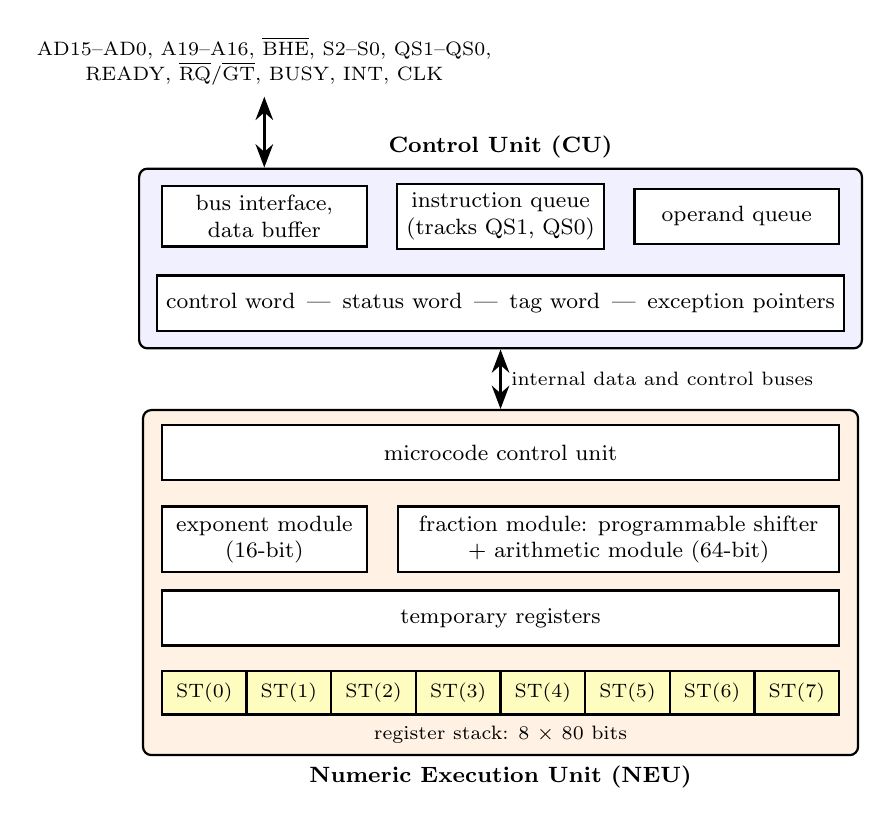
\begin{tikzpicture}[>=Stealth,font=\small,
 b/.style={draw,thick,fill=white,align=center,font=\footnotesize,minimum height=0.7cm}]
% control unit
\node[b,minimum width=2.6cm] (bi) at (0,0) {bus interface,\\data buffer};
\node[b,minimum width=2.6cm] (iq) at (3.0,0) {instruction queue\\(tracks QS1, QS0)};
\node[b,minimum width=2.6cm] (oq) at (6.0,0) {operand queue};
\node[b,minimum width=8.6cm] (regs) at (3.0,-1.1) {control word\enspace|\enspace status word\enspace|\enspace tag word\enspace|\enspace exception pointers};
\node[draw,thick,rounded corners=3pt,fill=blue!6,fit=(bi)(oq)(regs),inner sep=6pt,label={[font=\footnotesize\bfseries]above:Control Unit (CU)}] (cu) {};
\node[b,minimum width=2.6cm] at (0,0) {bus interface,\\data buffer};
\node[b,minimum width=2.6cm] at (3.0,0) {instruction queue\\(tracks QS1, QS0)};
\node[b,minimum width=2.6cm] at (6.0,0) {operand queue};
\node[b,minimum width=8.6cm] at (3.0,-1.1) {control word\enspace|\enspace status word\enspace|\enspace tag word\enspace|\enspace exception pointers};
% NEU
\begin{scope}[yshift=-3.6cm]
\node[b,minimum width=8.6cm] (mc) at (3.0,0.6) {microcode control unit};
\node[b,minimum width=2.6cm] (ex) at (0,-0.5) {exponent module\\(16-bit)};
\node[b,minimum width=5.6cm] (fr) at (4.5,-0.5) {fraction module: programmable shifter\\+ arithmetic module (64-bit)};
\node[b,minimum width=8.6cm] (tmp) at (3.0,-1.5) {temporary registers};
\foreach \i in {0,...,7} \node[draw,thick,fill=yellow!25,minimum width=1.075cm,minimum height=0.55cm,font=\scriptsize] at (-0.7625+\i*1.075,-2.45) {ST(\i)};
\node[font=\scriptsize,anchor=north] at (3.0,-2.75) {register stack: 8 $\times$ 80 bits};
\node[draw,thick,rounded corners=3pt,fill=orange!10,fit={(-1.4,1.0) (7.4,-3.1)},inner sep=4pt,label={[font=\footnotesize\bfseries]below:Numeric Execution Unit (NEU)}] (neu) {};
\node[b,minimum width=8.6cm] at (3.0,0.6) {microcode control unit};
\node[b,minimum width=2.6cm] at (0,-0.5) {exponent module\\(16-bit)};
\node[b,minimum width=5.6cm] at (4.5,-0.5) {fraction module: programmable shifter\\+ arithmetic module (64-bit)};
\node[b,minimum width=8.6cm] at (3.0,-1.5) {temporary registers};
\foreach \i in {0,...,7} \node[draw,thick,fill=yellow!25,minimum width=1.075cm,minimum height=0.55cm,font=\scriptsize] at (-0.7625+\i*1.075,-2.45) {ST(\i)};
\node[font=\scriptsize,anchor=north] at (3.0,-2.75) {register stack: 8 $\times$ 80 bits};
\end{scope}
\draw[<->,very thick] (cu.south) -- (neu.north) node[midway,right,font=\scriptsize]{internal data and control buses};
\draw[<->,very thick] (cu.north -| bi) -- ++(0,0.9) node[above,font=\scriptsize,align=center]{AD15--AD0, A19--A16, $\overline{\mathrm{BHE}}$, S2--S0, QS1--QS0,\\READY, $\overline{\mathrm{RQ}}$/$\overline{\mathrm{GT}}$, BUSY, INT, CLK};
\end{tikzpicture}
\end{document}
